\documentclass[UTF8]{ctexart}
\usepackage{amsmath}
\usepackage{amssymb}
\usepackage{booktabs}
\usepackage{background}
\usepackage{caption,subcaption}
\usepackage{CJKfntef}
\usepackage{cprotect}
\usepackage{enumitem}
\usepackage{fancyhdr}
\usepackage{float}
\usepackage{fontspec}
%\usepackage{fourier}
\usepackage{geometry}
\usepackage{listings}
\usepackage{tcolorbox}
\tcbuselibrary{breakable}
\usepackage{tikz}
\usetikzlibrary{arrows.meta}
\usepackage[table]{xcolor}

\geometry{a5paper, top=0.1cm, left=1cm, right=1cm, bottom=1cm, footskip=0.1cm}
\setCJKmainfont[BoldFont={汉仪文黑-85W},ItalicFont={方正苏新诗柳楷简体}]{汉仪文黑-55W}
\setfontfamily\Issue{Century Schoolbook}
\setfontfamily\Genshin{Genshin Teyvat Lingua Franca}
\newCJKfontfamily\TitleFont{思源宋体 CN Heavy}
\newfontfamily\timesnewroman{Times New Roman}
%\reversemarginpar

\pagestyle{fancy}
\fancyhf{}
\cfoot{\sffamily\footnotesize{-\ \thepage\ -}}
%\CTEXsetup[format = {\centering\bfseries\large}, beforeskip = 3pt, afterskip = 3pt]{section}

\colorlet{darkcyan}{cyan!50!black}
\newcommand\Black[1]{\textcolor[gray]{0.3}{#1}}
\newcommand\Brown[1]{\textcolor[HTML]{998A4E}{#1}}
\newcommand\Emph[1]{\colorbox{green!10}{\textcolor{green!30!black}{#1}}}
\newcommand\Notes[1]{\textcolor{yellow!50!black}{\small #1}}
\newcommand\Example[1]{\textcolor{cyan!70!black}{\small #1}}
\newcommand\keyword[1]{\textcolor{violet}{\textbf{\texttt{#1}}}}

\newtcolorbox{mybox}[1][内容概述]{colback=teal!10, colframe=teal!50!black, boxrule=1pt, title={#1}}

\renewcommand\d{\mathrm{d}}

\lstset{
    basicstyle=\small\ttfamily, %注意行末有逗号!
    keywordstyle=\bfseries\color{blue!70!black},
    commentstyle=\color{cyan!90!black},
    stringstyle=\color{green!40!black},
    columns=flexible,
    numbers=left,
    numberstyle=\footnotesize,
    escapechar=`,
    frame=shadowbox,
    %rulesepcolor=\color{red!20!blue!20!green!20}
    backgroundcolor=\color{cyan!5!white},
    language = C++,
    tabsize = 4,
    breaklines = true,
    showstringspaces = false,
}

\newcommand\IssueNumber{33}
\newcommand\Date{2024-9-13}
%\newcommand\Contributer{@金光日}
\newcommand\Subject{计算机网络}


\begin{document}
\backgroundsetup{contents=
\includegraphics{上半示例.png}, center, scale=1, angle=0, opacity=1}
\BgThispage
\begin{center}
%{\scriptsize\Issue \textcolor[HTML]{C8BA83}{\Genshin WEEKLY TIPS}}
\phantom{...}

{\Large\textcolor{brown!40!white}{\makebox[10cm][s]{\Genshin WEEKLY KNOWLEDGE TIPS}}}

\vspace{-2em}

{\Huge\bfseries\TitleFont \Black{知\ 识\ 小\ 料}}


\vspace{-0.1cm}
{\footnotesize \Brown{「电计 2203 班」周常规知识整理共享}}
\end{center}

\vspace{-0.5cm}


\begin{figure}[H]
\hspace{1cm}
\begin{minipage}[t]{0.3\textwidth}
\centering
    \Brown{\Genshin ISSUE}

    \vspace{-0.6cm}
    \Huge \Issue\slshape\bfseries\Black{\IssueNumber}
\end{minipage}
\hfill
\begin{minipage}[t]{0.35\textwidth}
\centering
    \Brown{日期:\Date} \\
%\vspace{-0.1cm}
%    \Brown{贡献者:\Contributer} \\
\vspace{-0.1cm}
    \Brown{学科:\Subject} \\
\end{minipage}
\hspace{0.8cm}
\end{figure}

{\color{cyan!50!black}
本文档列出了计算机网络前四节课知识要点梗概。
}

\part{计算机网络总体内容}
\begin{mybox}
本部分内容包括:
\begin{enumerate}[itemsep=0pt,parsep=0pt]
  \item 网络与协议的介绍
  \item 网络边缘:主机、接入网、物理媒体
  \item 网络核心:分组交换、电路交换
  \item 网络结构:「网络的网络」
  \item 网络性能:延迟、丢包、吞吐量
  \item 协议栈分层
\end{enumerate}
\end{mybox}

\section{网络与协议的介绍}
网络由设备、交换机、通信链路构成。因特网是「网络的网络」。

协议:定义了网络实体之间收发消息的格式、顺序,以及收发报文或其他时间所采取的操作。协议的三个要素是:\Emph{语法、语义、同步(或时序)}。

整个互联网划分为边缘部分和核心部分。

无线接入网有无线局域网(WLAN)和广域蜂窝接入网等。

\section{网络边缘}
网络边缘有\textbf{客户端}(client)和\textbf{服务器}(server)。或分为主机、接入网络、物理媒介。

主机发送数据包的传输延迟等于 $\dfrac{\text{数据长度}}{\text{传输速率}} = \dfrac{L_{\text{(bits)}}}{R_{\text{(bits/s)}}}$(单位:s)

网络边缘有两种通信方式:
\begin{itemize}[itemsep=0pt,parsep=0pt]
  \item 客户—服务器方式(Client-Server, C-S)
  \item 对等方式(Peer-to-Peer, P2P)
\end{itemize}

\backgroundsetup{contents=
\includegraphics{空白示例.png}, center, scale=1, angle=0, opacity=1}
\BgThispage
\section{网络核心}
网络核心有\textbf{交换机}和\textbf{数据链路}。其中交换机也叫做网络提供商(Internet Service Provider, ISP)。

网络报文交换分为两种方式:
\begin{itemize}[itemsep=0pt,parsep=0pt]
  \item \textbf{分组交换}。这是交换机将数据包\underline{存储、转发、传输}的一种方式。整个数据包需要完全到达路由器才能开始下一轮传输。数据包可能会排队、丢失。

  \item \textbf{电路交换}。相当于单开一条从起点到终点的专属电路来进行报文交换。分为\underline{频分复用}(FDM)和\underline{时分复用}(TDM)两种类型。
\end{itemize}

\section{网络结构}
因特网是「网络的网络」。

在全球的网络中,只有网络提供商(ISP)还不够,可能需要辗转于几个大的 ISP 之间的网络交换点(Internet Exchange Point, IXP)。

\section{延迟、吞吐量}
在\textbf{分组交换}中,数据包可能会延迟、丢包。

网络延迟由四部分组成:$d_{\text{nodal}} = d_{\text{proc}} + d_{\text{queue}} + d_{\text{trans}} + d_{\text{prop}}$。
\begin{enumerate}[itemsep=0pt,parsep=0pt]
  \item $d_{\text{proc}}$:处理(processing),数据包在节点里等待处理的用时
  \item $d_{\text{queue}}$:排队(queue),数据包排队时的时间
  \item $d_{\text{trans}}$:传输(transmission),数据包从节点「发出去」用时
  \item $d_{\text{prop}}$:传播(propagation),数据包从节点送到另一节点的用时,较长
\end{enumerate}

\begin{figure}[htb]
  \centering
  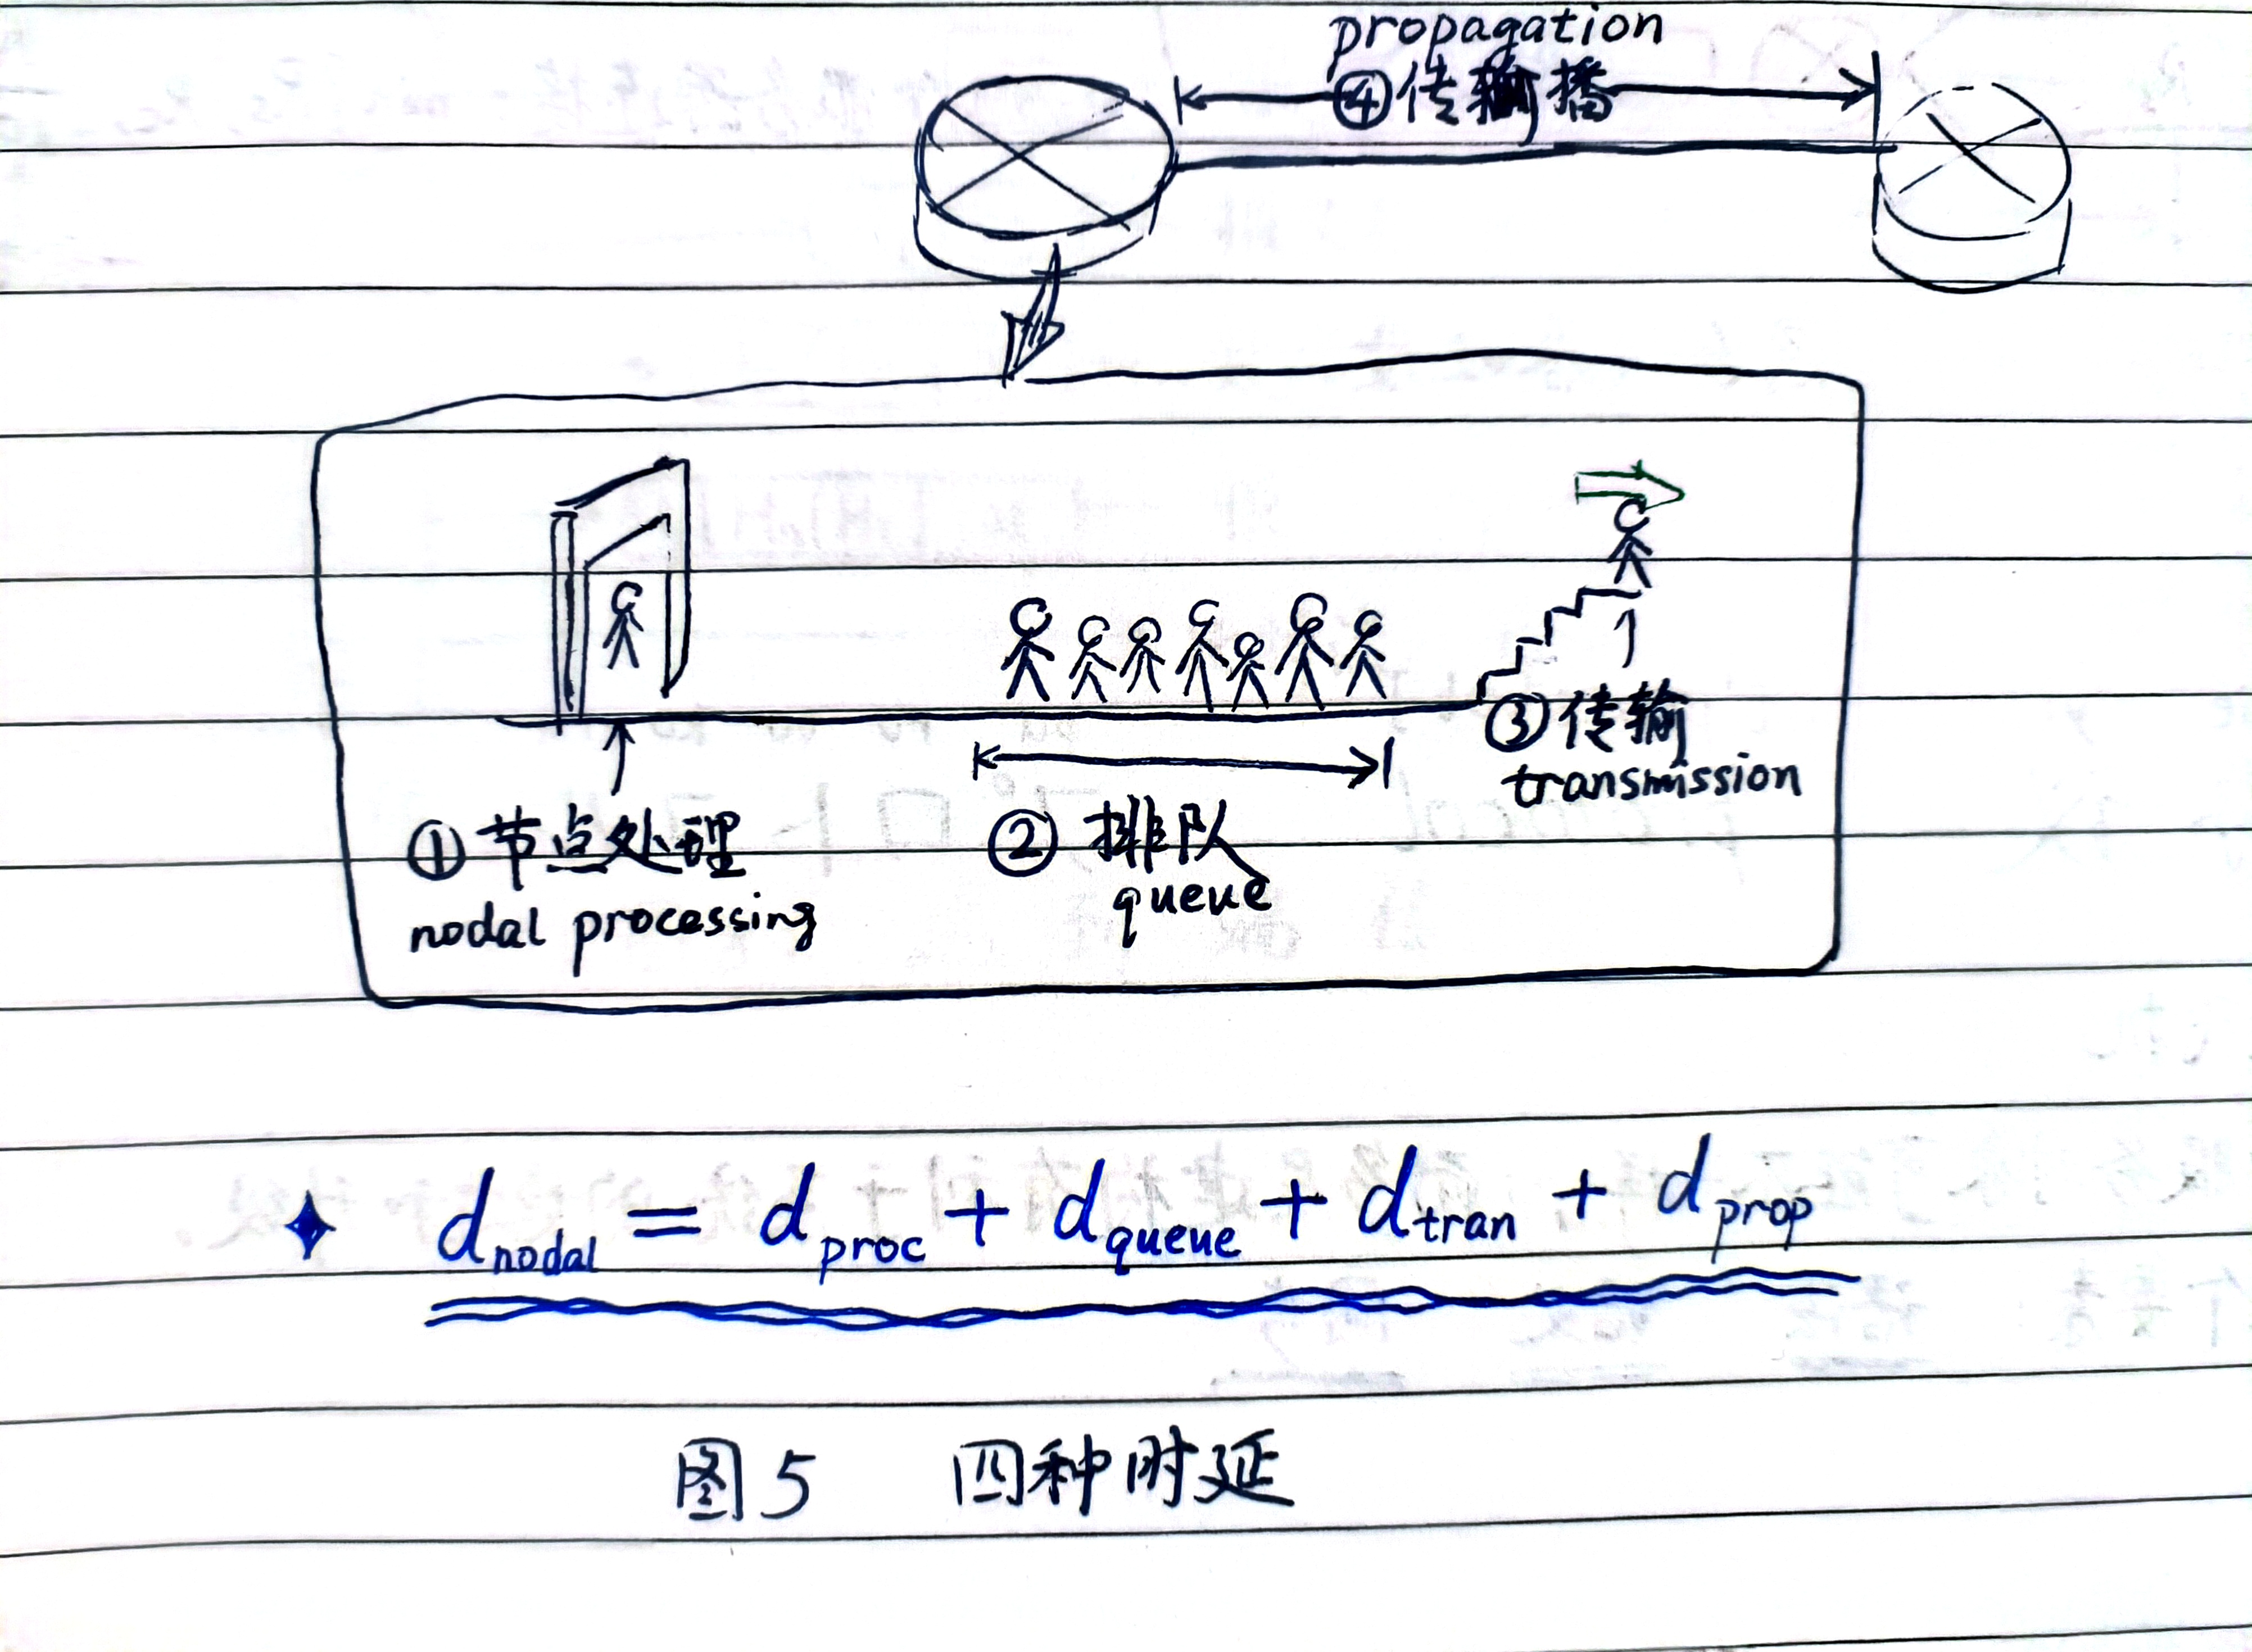
\includegraphics[width=6cm]{四种时延.jpg}
  \caption{分组交换的四部分时延图解(摘自课堂笔记)}\label{fig:四种时延}
\end{figure}

时延与网络利用率的关系:利用率 $La/R$ 趋于 1 则时延迅速增加,大于 1 则开始拥堵。

吞吐量(Throughput)表示单位时间内传输的字节数:$\dfrac{\text{字节数}}{\text{用时}}$(单位:bit/s)

当发送端吞吐量 $R_s$ 和接收端吞吐量 $R_c$ 不一样时,总吞吐量依据「短板效应」取较小者:$\min\{R_s,R_c\}$。

\section{协议栈分层}
\begin{table}[htb]
  \centering
  \begin{tabular}{ccccc}
  \toprule
  序号 & 名称 & 英文名 & 作用 & 相关协议 \\
  \midrule
  1 & 应用层 & Application & 支持应用 & HTTP, FTP, DNS 等 \\
  2 & 传输层 & Transport & 数据传输 & TCP, UDP \\
  3 & 网络层 & Network & 源到目标之路由 & IP \\
  4 & 链路层 & Link & 网络间连接 & 802.11(WiFi) \\
  5 & 物理层 & Physical & 比特流动 & 没什么协议 \\
  \bottomrule
  \end{tabular}
  \caption{协议栈分层}\label{tab:协议栈分层}
\end{table}

报文在各个层级间传递时,名称也不尽相同:
\begin{enumerate}[itemsep=0pt,parsep=0pt]
  \item 在应用层:报文(message)
  \item 在传输层:报文段(segment)
  \item 在网络层:数据报(datagram)
  \item 在链路层:帧(frame)
\end{enumerate}

最后,可以用 \verb!tracert! 命令观察一个 IP 地址经历了多少路由器。


\part{应用层}
\begin{mybox}
本部分内容包括:
\begin{enumerate}[itemsep=0pt,parsep=0pt]
  \item 应用层总体介绍
  \item Web 服务和 HTTP 协议、万维网的工作流程
  \item 域名解析系统(DNS)
\end{enumerate}
\end{mybox}

\section{应用层总体介绍}
应用层对标的是端系统;网络核心设备不含应用层。

应用进程间的服务模式:
\begin{itemize}
  \item 客户—服务器模式(C-S):客户端间歇性连接;服务器需要一直打开。

  主要支持协议有 HTTP, FTP, DNS, Web 协议等。

  \item 对等模式(P2P):主要支持协议:BT 种子等。
\end{itemize}

进程通信协议采用「套接字」(socket)。进程 = IP 地址 + 端口号。

网络运输服务分为 TCP 和 UDP 两种。

安全的 TCP 可能会使用虚拟的「安全套接字层」(SSL)。

\section{Web 服务与 HTTP 协议}
WWW 又称万维网(World Wide Web),简称 Web。它以\textbf{客户—服务器模式}工作。

万维网的工作大致流程:
\begin{enumerate}[itemsep=0pt,parsep=0pt]
  \item 输入 URL
  \item 浏览器向域名系统(DNS)请求解析地址
  \item DNS 解析出来了 IP 地址
  \item 浏览器与服务器建立 TCP 连接
  \item 浏览器发出 HTTP 请求报文,服务器返回 HTTP 响应报文
  \item 释放 TCP 连接
\end{enumerate}

HTML 即超文本标记语言,简单易上手,成品如老师的随机点名网站。

HTTP 即超文本传输协议:
\begin{itemize}[itemsep=0pt,parsep=0pt]
  \item 不持续的 HTTP:报文响应时间$ = 2\times RTT + $文件传输时间。
  \item 持续的 HTTP——HTTP1.1:能保持连接,弊端是队头拥堵(HOL blocking)。
  \item HTTP2:把文件分割成帧传输,不拥堵,弊端是安全性不够
  \item HTTP3:如今的版本
\end{itemize}

HTTP 的请求和响应报文有特定的格式,也有如 404、200 等返回状态值。

保持连接顺畅的利器:Cookie

加速连接的代理服务器:网络缓存(cache)

\section{域名解析系统}
域名解析系统(DNS)是一种映射表,用于建立从域名到 IP 地址的映射。

因特网的域名呈树状结构,格式为从低级写到高级。\verb!mail.dlut.edu.cn! 中,\verb!mail! 是四级域名,\verb!dlut! 是三级域名,\verb!edu! 是二级域名,\verb!cn! 是一级域名。

将域名转换为 IP 地址的过程称为域名解析。

本地域名服务器采用迭代查询或递归查询的方式。

\newpage
\backgroundsetup{contents=
\includegraphics{下半示例.png}, center, scale=1, angle=0, opacity=1}
\BgThispage
\vspace{0pt}

\begin{tcolorbox}[tabulars={@{\extracolsep{\fill}\hspace{5mm}}ccc@{\hspace{5mm}}},
boxrule=0.5pt,title=英语缩略词表, breakable,  fonttitle=\bfseries, colback = violet!5, colframe = violet!70!black, center title, ]
    英文简称 & 英文全称 & 中文全称 \\ \hline\hline
    
    C-S & Client-Server & 客户—服务器通信模式 \\ \hline
    DNS & Domain Name System & 域名解析系统 \\ \hline
    FDM & Frequency-Division Multiplexing & 频分复用 \\ \hline
    FTP & File Transfer Protocol & 文件传输协议 \\ \hline
    HTML & Hypertext Markup Language & 超文本标记语言 \\ \hline
    HTTP & Hypertext Transfer Protocol & 超文本传输协议 \\ \hline
    IP & Internet Protocol & 互联网协议 \\ \hline
    ISP & Internet Service Provider & 网络提供商 \\ \hline
    IXP & Internet Exchange Point & 网络交换点 \\ \hline
    P2P & Peer-to-Peer & 对等通信模式 \\ \hline
    TCP & Transmission Control Protocol & 传输控制协议 \\ \hline
    TDM & Time-Division Multiplexing & 时分复用 \\ \hline
    UDP & User Datagram Protocol & 用户数据报协议 \\ \hline
    WLAN & Wireless Local Area Network & 无线局域网 \\ \hline
    WWW & World Wide Web & 万维网 \\ 
    
\end{tcolorbox}


\end{document} 